\chapter{Probabilités}

\section{Problème des deux enfants}

\subsection*{Exercice :}
 
\begin{exerciseBox}[Problème des deux enfants]
Une femme a deux enfants. Sachant que l'un d'eux est une fille, calculer la probabilité que l'autre soit un garçon.
\end{exerciseBox}

\subsection*{Solution :}

Notons
\[
A : \{\text{l'autre enfant est un garçon}\}, \qquad
B : \{\text{il y a au moins une fille}\}.
\]
On cherche donc
\[
P(A \mid B).
\]
Par le théorème de Bayes,
\[
P(A \mid B) = \frac{P(A \cap B)}{P(B)}.
\]

Les couples possibles pour les deux enfants sont
\[
\Omega = \{GG,\; GF,\; FG,\; FF\},
\]
tous équiprobables, de probabilité $\tfrac14$.

\begin{itemize}
\item $B = \{GF, FG, FF\}$, donc $P(B) = \tfrac34$.
\item $A \cap B$ correspond au fait qu’il y a au moins une fille et l’autre est un garçon,
      c’est-à-dire $\{GF, FG\}$, donc $P(A \cap B) = \tfrac12$.
\end{itemize}

Ainsi,
\[
P(A \mid B)
= \frac{P(A \cap B)}{P(B)}
= \frac{\tfrac12}{\tfrac34}
= \boxed{\tfrac{2}{3}}.
\]



\section{Deux lancers de dé}

\subsection*{Exercice :}

\begin{exerciseBox}[Deux lancers de dé]
On lance un dé équilibré à six faces deux fois successivement.
Calculer la probabilité que la valeur obtenue au premier lancer soit strictement inférieure à celle obtenue au second lancer.
\end{exerciseBox}

\subsection*{Solution :}

Notons les résultats des deux lancers $X_1$ et $X_2$.
L’espace des possibles est
\[
\Omega=\{1,2,3,4,5,6\}^2,
\]
de cardinal $36$, tous les couples étant équiprobables.

Nous cherchons
\[
P\bigl(X_1 < X_2\bigr)
= \frac{\text{nombre de couples }(x_1,x_2)\text{ tels que }x_1<x_2}{36}.
\]

Pour chaque valeur de $x_2$, le nombre de valeurs de $x_1$ plus petites est $x_2-1$.
Ainsi
\[
\#\{x_1<x_2\}
= \sum_{x_2=1}^6 (x_2-1)
= 0+1+2+3+4+5
= 15.
\]

Donc
\[
P(X_1 < X_2)
= \frac{15}{36}
= \frac{5}{12}.
\]




\section{Pièce biaisée}

\subsection*{Exercice :}

\begin{exerciseBox}[Pièce biaisée]
On dispose d’un ensemble de $100$ pièces : une seule est biaisée et possède deux faces « pile »,
les $99$ autres sont des pièces équilibrées.\\
On choisit une pièce au hasard et on la lance $10$ fois.
Elle tombe « pile » à chaque lancer.
Calculer la probabilité que la pièce choisie soit la pièce biaisée.
\end{exerciseBox}

\subsection*{Solution :}


Soit
\[
U : \{\text{la pièce choisie est la pièce biaisée}\}, 
F : \{\text{la pièce choisie est une pièce équilibrée}\},
\]
\[
H : \{\text{les 10 lancers donnent pile}\}.
\]

Les probabilités a priori sont
\[
P(U) = \frac{1}{100}, \qquad
P(F) = \frac{99}{100}.
\]
Par la formule de Bayes,
\[
P(U \mid H)
= \frac{P(H \mid U)\,P(U)}
       {P(H \mid U)\,P(U) + P(H \mid F)\,P(F)}.
\]


or  :
\[
P(H \mid U) = 1,
\qquad
P(H \mid F) = \left(\frac{1}{2}\right)^{10}.
\]


En remplaçant les valeurs,
\[
P(U \mid H)
= \frac{1 \times \tfrac{1}{100}}
       {1 \times \tfrac{1}{100} + \left(\tfrac{1}{2}\right)^{10} \times \tfrac{99}{100}}
= \frac{1}{1 + 99\left(\tfrac{1}{2}\right)^{10}}.
\]

Comme $\left(\tfrac{1}{2}\right)^{10} = \tfrac{1}{1024}$, on obtient
\[
P(U \mid H)
= \frac{1}{1 + \dfrac{99}{1024}}
= \frac{1024}{1024 + 99}
= \boxed{\dfrac{1024}{1123}}.
\]


\section{Parité du nombre de piles}

\subsection*{Exercice :}

\begin{exerciseBox}[Parité du nombre de piles]
On lance $4$ pièces équilibrées et indépendantes. Quelle est la probabilité que le nombre de piles obtenues soit \emph{pair} ?
\end{exerciseBox}

\subsection*{Solution :}

Notons $X$ le nombre de piles. Alors $X \sim \mathrm{Bin}(4,\tfrac12)$.
On cherche $\mathbb{P}(X \in \{0,2,4\})$ :
\[
\mathbb{P}(X \in \{0,2,4\})
= \frac{\binom{4}{0} + \binom{4}{2} + \binom{4}{4}}{2^4}
= \frac{1+6+1}{16}
= \frac{8}{16}
= \boxed{\tfrac12}.
\]

\medskip
\textit{Variante (parité générale).} Pour $n$ lancers (avec $n$ pair),
\[
\sum_{k \text{ pair}} \binom{n}{k}
= \sum_{k \text{ impair}} \binom{n}{k}
= 2^{n-1},
\]
d’où $\mathbb{P}(\text{nombre de piles pair})=\frac{2^{n-1}}{2^n}=\tfrac12$.



\section{Élément choisi au hasard}

\subsection*{Exercice :}

\begin{exerciseBox}[Élément choisi au hasard]
On considère l’ensemble $\{1,2,\dots,n\}$.  
On choisit uniformément un élément $I$ dans cet ensemble.  
On définit
\[
X_1 = \#\{\text{éléments strictement inférieurs à } I\},
X_2 = \#\{\text{éléments strictement supérieurs à } I\}.
\]
Calculer l’espérance $\mathbb{E}[X_1]$.
\end{exerciseBox}


\subsection*{Solution :}

L’élément choisi $I$ est uniforme sur $\{1,2,\dots,n\}$, donc
\[
P(I = k) = \frac{1}{n}, \qquad k=1,\dots,n.
\]
Par définition,
\[
X_1 = \#\{j \in \{1,\dots,n\} : j < I\} = I - 1.
\]

d'où $X_1$ a valeurs dans $\{0,1,\dots,n-1\}$

Ainsi
\[
\mathbb{E}[X_1]
= \sum_{k=0}^{n-1} k \, P(X_1=k) 
= \sum_{k=1}^{n} (k-1) \, P(I=k) 
= \frac{1}{n} \sum_{k=1}^n (k-1).
\]



Or
\[
\sum_{k=1}^n (k-1) = \sum_{m=0}^{\,n-1} m
= \frac{(n-1)n}{2}.
\]

Donc
\[
\mathbb{E}[X_1]
= \frac{1}{n} \cdot \frac{n(n-1)}{2}
= \boxed{\displaystyle \frac{n-1}{2}}.
\]




\section{Premier As}

\subsection*{Exercice :}

\begin{exerciseBox}[Premier As]
En moyenne, combien de cartes faut-il retourner dans un jeu standard de 52 cartes
pour observer le premier As ?
\end{exerciseBox}

\subsection*{Solution :}

introduisons les variables suivantes :

\[
X_1 = \#\{\text{cartes avant le 1er As}\}, \quad
X_2 = \#\{\text{cartes entre le 1er et le 2e As}\}, \quad
\]

\[
X_3 = \#\{\text{cartes entre le 2e et le 3e As}\},
X_4 = \#\{\text{cartes entre le 3e et le 4e As}\},
X_5 = \#\{\text{cartes après le 4e As}\}.
\]

Ces cinq variables comptent le nombre de cartes
entre deux As successifs (ou avant le premier et après le dernier).
On a évidemment
\[
X_1 + X_2 + X_3 + X_4 + X_5 = 52 - 4 = 48
\]
puisque seules les cartes \emph{non As} sont comptées dans les intervalles.

\medskip
\textbf{Symétrie du mélange.}

Le mélange est parfaitement uniforme.
Les quatre As découpent les 48 autres cartes en 5 « blocs »
séparés par les As.
Par symétrie, les intervalles
\((X_1,X_2,X_3,X_4,X_5)\)
ont même espérance :
\[
\mathbb{E}[X_1] = \mathbb{E}[X_2] = \mathbb{E}[X_3]
= \mathbb{E}[X_4] = \mathbb{E}[X_5].
\]

\paragraph{Espérance de chaque $X_i$.}

Définissons les indicatrices :
\[
I_{j,i} = \mathbf{1}_{\{\text{la $j$-ième carte non-As est dans l’intervalle $i$}\}}.
\]

Alors
\[
X_i = \sum_{j=1}^{48} I_{j,i}.
\]

Or
\[
\mathbb{E}[I_{j,i}] = P(C_j \in X_i) = \frac{1}{5}.
\]

Donc
\[
\mathbb{E}[X_i]
= \sum_{j=1}^{48} \mathbb{E}[I_{j,i}]
= 48 \times \frac{1}{5}
= \frac{48}{5}.
\]

d’où
\[
\boxed{
\mathbb{E}[X_i]  = \frac{48}{5} 
} \quad \forall i \in \{1,2,3,4,5\}\]

\medskip
\textbf{Position du premier As.}

La position $N$ du premier As est
\[
N = X_1 + 1
\]
(car il y a $X_1$ cartes non As avant, puis le premier As).

Ainsi
\[
\mathbb{E}[N]
= \mathbb{E}[X_1] + 1
= \frac{48}{5} + 1
= \frac{48 + 5}{5}
= \boxed{\displaystyle \frac{53}{5}}.
\]

\medskip
Numériquement,
\[
\mathbb{E}[N] \approx 10,6.
\]


\section{Minimum de $k$ positions}

\subsection*{Exercice :}

\begin{exerciseBox}[Minimum de $k$ positions]
On choisit $k$ positions distinctes de manière uniforme parmi l’ensemble
$\{1,2,\dots,n\}$.
Notons
\[
M = \min\{X_1,\dots,X_k\}
\]
le minimum des positions choisies.
Calculer l’espérance $\mathbb{E}[M]$.
\end{exerciseBox}

\subsection*{Solution :}


On choisit $k$ positions distinctes de manière uniforme parmi $\{1,2,\dots,n\}$.
Notons $M = \min\{X_1,\dots,X_k\}$ leur minimum.

\medskip
\textbf{1. Distribution de $M$.}

On a
\[
P(M > m) = P(\text{tous les $k$ éléments sont dans } \{m+1,\dots,n\}).
\]
Le nombre de façons de choisir $k$ éléments dans $\{m+1,\dots,n\}$ est
\(\binom{n-m}{k}\).
Le nombre total de $k$-ensembles dans $\{1,\dots,n\}$ est
\(\binom{n}{k}\).
Donc
\[
P(M > m) = \frac{\binom{n-m}{k}}{\binom{n}{k}}, 
\qquad m=0,1,\dots,n-k.
\]

\medskip
\textbf{2. Formule de l'espérance.}

Par la formule générale
\[
\mathbb{E}[M] = \sum_{m=0}^{n-1} P(M > m).
\]
Donc
\[
\mathbb{E}[M] = \sum_{m=0}^{n-1} \frac{\binom{n-m}{k}}{\binom{n}{k}}.
\]

\medskip
\textbf{3. Changement d’indice.}

Posons $j = n-m$, alors $m=0 \Rightarrow j=n$, et $m=n-1 \Rightarrow j=1$.
Ainsi,
\[
\mathbb{E}[M] = \frac{1}{\binom{n}{k}} \sum_{j=1}^{n} \binom{j}{k}.
\]

\medskip
\textbf{4. Identité combinatoire.}

On utilise l’identité de \textbf{hockey-stick} :
\[
\sum_{j=k}^{n} \binom{j}{k} = \binom{n+1}{k+1}.
\]
Donc
\[
\mathbb{E}[M] = \frac{\binom{n+1}{k+1}}{\binom{n}{k}}.
\]

\medskip
\textbf{5. Simplification.}

On a
\[
\frac{\binom{n+1}{k+1}}{\binom{n}{k}}
= \frac{\frac{(n+1)!}{(k+1)!(n-k)!}}{\frac{n!}{k!(n-k)!}}
= \frac{n+1}{k+1}.
\]

\medskip
Ainsi,
\[
\boxed{\mathbb{E}[M] = \frac{n+1}{k+1}}.
\]






\section{Labyrinthe du rat}

\subsection*{Exercice :}

\begin{exerciseBox}[Labyrinthe du rat]
Un rat se trouve dans un labyrinthe, face à deux portes. À chaque tentative, il choisit :

\begin{itemize}
  \item la \textbf{première porte} avec une probabilité \( p \), et
  \item la \textbf{deuxième porte} avec une probabilité \( 1 - p \).
\end{itemize}

\begin{itemize}
  \item S’il choisit la \textbf{première porte}, il revient immédiatement à son point de départ après \textbf{une minute}.
  \item S’il choisit la \textbf{deuxième porte}, il se déplace vers un point intermédiaire en \textbf{une minute}, puis :
  \begin{itemize}
    \item il \textbf{rebrousse chemin} avec une probabilité \( q \), ce qui lui prend encore \textbf{une minute}, 
    \item ou il \textbf{quitte définitivement le labyrinthe} avec une probabilité \( 1 - q \), après \textbf{une minute}.
  \end{itemize}
\end{itemize}

Tous les choix du rat sont faits de manière indépendante les uns des autres.

\vspace{0.5em}
On note \( T \) le \textbf{temps total passé par le rat dans le labyrinthe}.\\

\textbf{Questions :}
\begin{enumerate}
  \item Déterminer l’espérance \( \mathbb{E}[T] \).
  \item Déterminer la loi de probabilité de \( T \).
\end{enumerate}
\end{exerciseBox}

\subsection*{Solution :}

% \section*{Solution par la formule de l'espérance conditionnelle}

On note \( T \) le temps total passé dans le labyrinthe. Le rat choisit :

\begin{itemize}
  \item la porte 1 avec une probabilité \( p \)
  \item la porte 2 avec une probabilité \( 1 - p \)
\end{itemize}

et soit $N$  le numéro de la porte choisie au départ du rat.
 

\subsection*{Cas 1 : Choix de la porte 1}

S'il choisit la porte 1, il revient au point de départ après 1 minute, et recommence exactement la même situation. Ainsi :
\[
\mathbb{E}[T \mid N = 1] = 1 + \mathbb{E}[T]
\]

\subsection*{Cas 2 : Choix de la porte 2}

S'il choisit la porte 2, il atteint un point intermédiaire. À partir de là :

\begin{itemize}
  \item Avec probabilité \( 1 - q \), il sort du labyrinthe après 2 minutes (1 aller + 1 sortie)
  \item Avec probabilité \( q \), il revient au point de départ en 2 minutes (1 aller + 1 retour), et recommence
\end{itemize}

Ainsi :
\[
\mathbb{E}[T \mid N = 2] = (1 - q) \cdot 2 + q \cdot (2 + \mathbb{E}[T]) = 2 + q \cdot \mathbb{E}[T]
\]

\subsection*{Formule de l'espérance totale}

On applique la formule de l'espérance conditionnelle :

\[
\mathbb{E}[T] = p \cdot \mathbb{E}[T \mid N = 1] + (1 - p) \cdot \mathbb{E}[T \mid N = 2]
\]

Substituons les expressions obtenues :

\[
\mathbb{E}[T] = p(1 + \mathbb{E}[T]) + (1 - p)(2 + q \cdot \mathbb{E}[T])
\]

Développons :

\[
\mathbb{E}[T] = p + p \cdot \mathbb{E}[T] + 2(1 - p) + q(1 - p) \cdot \mathbb{E}[T]
\]

\[
\mathbb{E}[T] = p + 2(1 - p) + \left(p + q(1 - p)\right) \cdot \mathbb{E}[T]
\]

Factorisons :

\[
\mathbb{E}[T] \cdot \left(1 - \left(p + q(1 - p)\right)\right) = p + 2(1 - p)
\]

\[
\Rightarrow \mathbb{E}[T] = \frac{p + 2(1 - p)}{1 - \left(p + q(1 - p)\right)}
= \frac{p + 2(1 - p)}{(1 - p)(1 - q)}
\]

\subsection*{Conclusion}

L'espérance du temps passé dans le labyrinthe est donnée par la formule générale :

\[
\boxed{
\mathbb{E}[T] = \frac{p + 2(1 - p)}{(1 - p)(1 - q)}
}
\]


\section{Trois points sur un cercle}

\subsection*{Exercice :}


\begin{exerciseBox}[Trois points sur un cercle]
On choisit indépendamment et uniformément trois points $P_1,P_2,P_3$ sur un cercle de centre $O$. Quelle est la probabilité que $O$ appartienne au triangle $P_1P_2P_3$ ? 
\end{exerciseBox}




\subsection*{Solution}

Un critère équivalent est que $O \in \triangle P_1P_2P_3$ si et seulement si les trois points ne sont pas contenus dans un même demi-cercle. Ainsi,
\[
\mathbb{P}\big(O \in \triangle P_1P_2P_3\big)
= 1 - \mathbb{P}(\text{les trois points sont dans un même demi-cercle}).
\]

Fixons $P_1$. Considérons le demi-cercle \emph{ouvert} de longueur $\pi$ partant de $P_1$ dans un sens donné.  
La probabilité que $P_2$ et $P_3$ tombent tous deux dans ce demi-cercle vaut
\[
\left(\tfrac{1}{2}\right)^2 = \tfrac{1}{4}.
\]

Définissons $E_i =$ ``les trois points sont contenus dans un demi-cercle dont l’extrémité est $P_i$''.  
Alors $\mathbb{P}(E_i)=1/4$. De plus, les événements $E_1,E_2,E_3$ sont \emph{disjoints} : en effet, si deux d’entre eux se réalisaient simultanément, on aurait deux demi-cercles disjoints contenant les trois points, ce qui est impossible.

Par conséquent,
\[
\mathbb{P}(\text{les trois points sont dans un même demi-cercle})
= \mathbb{P}(E_1 \cup E_2 \cup E_3)
= \sum_{i=1}^3 \mathbb{P}(E_i)
= 3 \times \tfrac{1}{4}
= \tfrac{3}{4}.
\]

Finalement,
\[
\boxed{\ \mathbb{P}\big(O \in \triangle P_1P_2P_3\big) = 1 - \tfrac{3}{4} = \tfrac{1}{4} \ }.
\]




\section{Variable à variance maximale dans [-1,1]}

\subsection*{Exercice :}

\begin{exerciseBox}[Variable à variance maximale dans \ensuremath{[-1,1]}]
Soit $\Gamma$ l'ensemble des variables aléatoires $X$ telles que $X \in [-1,1]$ p.s.  
Déterminer
\[
X^* \in \arg\max_{X \in \Gamma} \operatorname{Var}(X)
\]
\end{exerciseBox}

\subsection*{Solution :}

Pour toute variable aléatoire $X \in [-1,1]$ p.s., on a
\[
\operatorname{Var}(X) = \mathbb{E}[X^2] - \big(\mathbb{E}[X]\big)^2.
\]
Or $X^2 \leq 1$, donc $\mathbb{E}[X^2] \leq 1$. Ainsi
\[
\operatorname{Var}(X) \leq 1 - \big(\mathbb{E}[X]\big)^2 \leq 1.
\]

Pour atteindre l'égalité $\operatorname{Var}(X) = 1$, il faut que
\[
\mathbb{E}[X^2] = 1 
\quad \text{et} \quad 
\mathbb{E}[X] = 0.
\]
La condition $\mathbb{E}[X^2]=1$ avec $X^2 \leq 1$ impose $|X|=1$ p.s., donc $X \in \{-1,1\}$ p.s.  
Ensuite, la condition $\mathbb{E}[X]=0$ implique
\[
\mathbb{P}(X=1)=\mathbb{P}(X=-1)=\tfrac{1}{2}.
\]

Ainsi, un maximiseur est la variable de \textbf{Rademacher} symétrique :
\[
X^* =
\begin{cases}
1, & \text{avec probabilité } \tfrac12, \\[6pt]
-1, & \text{avec probabilité } \tfrac12,
\end{cases}
\qquad \text{et} \qquad \operatorname{Var}(X^*)=1.
\]

\medskip
\textbf{Remarque.} Plus généralement, si $X \in [a,b]$ p.s., on a l'inégalité de Popoviciu :
\[
\operatorname{Var}(X) \leq \frac{(b-a)^2}{4},
\]
avec égalité pour $\mathbb{P}(X=a)=\mathbb{P}(X=b)=\tfrac12$.



\section{Somme de variables uniformes}
\begin{exerciseBox}[Somme de variables uniformes]
Soient \( X_1, X_2, \dots \) une suite de variables aléatoires indépendantes et identiquement distribuées, suivant la loi uniforme \( \mathcal{U}[0,1] \).

On définit :
\[
N := \min \left\{ n \geq 1 \mid \sum_{i=1}^n X_i > 1 \right\}
\]

Autrement dit, \( N \) est le nombre de tirages nécessaires pour que la somme dépasse 1.

\vspace{0.5em}
\textbf{Question :} Déterminer l'espérance \( \mathbb{E}[N] \).
\end{exerciseBox}

\subsection*{Solution :}


On utilise la formule générale de l'espérance pour une variable aléatoire à valeurs entières positives :

\[
\mathbb{E}[N] = \sum_{n=1}^\infty \mathbb{P}(N \geq n) = \sum_{n=0}^\infty \mathbb{P}(N > n)
\]

Or, par définition de \( N \), on a :
\[
\mathbb{P}(N > n) = \mathbb{P} \left( \sum_{i=1}^n X_i \leq 1 \right)
\]

Posons :
\[
P_n := \mathbb{P} \left( \sum_{i=1}^n X_i \leq 1 \right)
\]

Alors :
\[
\mathbb{E}[N] = \sum_{n=0}^\infty P_n
\]


\subsection*{Calcul de \( P_n \)}

On cherche :
\[
P_n = \mathbb{P}\left( X_1 + \dots + X_n \leq 1 \right)
= \int_{[0,1]^n} \mathbf{1}_{\{x_1 + \cdots + x_n \leq 1\}} \, dx_1 \cdots dx_n
\]

Ce domaine est le \textbf{simplexe} :
\[
\Delta_n := \left\{ (x_1, \dots, x_n) \in [0,1]^n \mid \sum x_i \leq 1 \right\}
\]

Ce simplexe a un volume connu :
\[
\text{Vol}(\Delta_n) = \frac{1}{n!}
\]

\textit{(ce résultat classique peut se montrer par récurrence ou en intégrant successivement sur \( x_1, \dots, x_n \))}

\subsection*{Conclusion}

On a donc :
\[
\mathbb{E}[N] = \sum_{n=0}^\infty \frac{1}{n!} = e
\]

\vspace{0.5em}
\[
\boxed{ \mathbb{E}[N] = e }
\]


\subsection*{Illustration géométrique du simplexe pour \( n = 2 \)}

Pour \( n = 2 \), on considère :
\[
P_2 = \mathbb{P}(X_1 + X_2 \leq 1) = \int_{[0,1]^2} \mathbf{1}_{\{x + y \leq 1\}} \, dx \, dy
\]

Le domaine d'intégration est le triangle ci-dessous, de sommet \( (0,0), (1,0), (0,1) \), formant un simplexe de dimension 2.

\vspace{1em}

\begin{center}
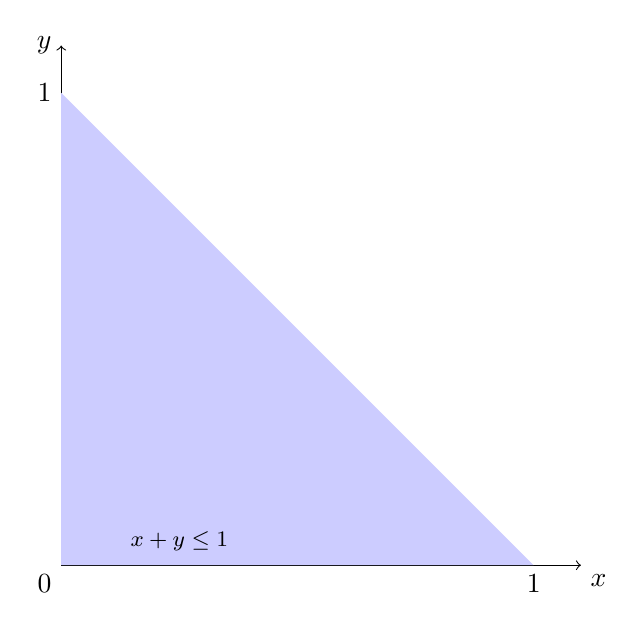
\begin{tikzpicture}[scale=6]
  % Axes
  \draw[->] (0,0) -- (1.1,0) node[below right] {\( x \)};
  \draw[->] (0,0) -- (0,1.1) node[left] {\( y \)};

  % Triangle
  \fill[blue!20] (0,0) -- (1,0) -- (0,1) -- cycle;

  % Labels
  \node[below left] at (0,0) {\( 0 \)};
  \node[below] at (1,0) {\( 1 \)};
  \node[left] at (0,1) {\( 1 \)};
  \node at (0.25,0.05) {\footnotesize \( x + y \leq 1 \)};
\end{tikzpicture}

\captionof{figure}{Domaine \( \{(x, y) \in [0,1]^2 \mid x + y \leq 1\} \), volume \( \frac{1}{2} \)}
\end{center}

\vspace{1em}

On voit que l’aire du triangle est :
\[
\text{Aire} = \frac{1}{2} = \frac{1}{2!}
\]

Cela confirme le fait que :
\[
P_2 = \frac{1}{2!}
\quad \text{et plus généralement} \quad
P_n = \frac{1}{n!}
\]


\section{Indépendance entre \(|X|\) et \(\mathrm{sign}(X)\) pour une loi normale}
\begin{exerciseBox}[Indépendance entre \(|X|\) et \(\mathrm{sign}(X)\) pour une loi normale]
Soit \( X \sim \mathcal{N}(0, 1) \). On note :
\[
\mathrm{sign}(X) =
\begin{cases}
+1 & \text{si } X >= 0 \\
-1 & \text{si } X < 0
\end{cases}
\]

\textbf{Question :} Montrer que les variables aléatoires \( |X| \) et \( \mathrm{sign}(X) \) sont indépendantes.
\end{exerciseBox}


\subsection*{Solution :}



Soit \( X \sim \mathcal{N}(0,1) \). On pose :
\[
Y := |X|, \quad S := \mathrm{sign}(X) =
\begin{cases}
+1 & \text{si } X \geq 0 \\
-1 & \text{si } X < 0
\end{cases}
\]

\vspace{0.5em}
Objectif :
\[
\forall y > 0,\ s \in \{-1, 1\} \quad
\mathbb{P}(Y \leq y,\ S = s) = \mathbb{P}(Y \leq y)\cdot \mathbb{P}(S = s)
\]


\subsection*{Étape 1 : Calcul de \( \mathbb{P}(Y \leq y, S = 1) \)}

\[
\mathbb{P}(Y \leq y, S = 1) = \mathbb{P}(0 \leq X \leq y) = \Phi(y) - \Phi(0)
\]

\[
\Phi(0) = \frac{1}{2} \Rightarrow \mathbb{P}(Y \leq y, S = 1) = \Phi(y) - \frac{1}{2}
\]

\subsection*{Étape 2 : Calcul de \( \mathbb{P}(Y \leq y)\cdot \mathbb{P}(S = 1) \)}



\textbf{Calcul de \( \mathbb{P}(Y \leq y) \)}

\[
\mathbb{P}(Y \leq y) = \mathbb{P}(-y \leq X \leq y) = \Phi(y) - \Phi(-y)
\]

\[
\text{Or } \Phi(-y) + \Phi(y) = 1 \Rightarrow \mathbb{P}(Y \leq y) = 2\Phi(y) - 1
\]

\textbf{Calcul de \( \mathbb{P}(S = 1)\)}


\[
\mathbb{P}(S = 1) = \mathbb{P}(X \geq 0) = 1 - \Phi(0) = \frac{1}{2}
\]

\[
\mathbb{P}(Y \leq y)\cdot \mathbb{P}(S = 1) = \left(2\Phi(y) - 1\right)\cdot \frac{1}{2} = \Phi(y) - \frac{1}{2}
\]

\[
\Rightarrow \mathbb{P}(Y \leq y, S = 1) = \mathbb{P}(Y \leq y)\cdot \mathbb{P}(S = 1)
\]

\subsection*{De même, pour \( S = -1 \) :}

\[
\mathbb{P}(Y \leq y, S = -1) = \mathbb{P}(-y \leq X < 0) = \Phi(0) - \Phi(-y)
\]

\[
\Phi(-y) = 1 - \Phi(y) \Rightarrow \Phi(0) - \Phi(-y) = \frac{1}{2} - (1 - \Phi(y)) = \Phi(y) - \frac{1}{2}
\]

\[
\mathbb{P}(Y \leq y)\cdot \mathbb{P}(S = -1) = (2\Phi(y) - 1)\cdot \frac{1}{2} = \Phi(y) - \frac{1}{2}
\]

\[
\Rightarrow \mathbb{P}(Y \leq y, S = -1) = \mathbb{P}(Y \leq y)\cdot \mathbb{P}(S = -1)
\]

\subsection*{Conclusion}

\[
\forall y > 0,\ \forall s \in \{-1, +1\},\quad \mathbb{P}(Y \leq y, S = s) = \mathbb{P}(Y \leq y)\cdot \mathbb{P}(S = s)
\Rightarrow Y \perp S
\]

\[
\boxed{ |X| \text{ et } \mathrm{sign}(X) \text{ sont indépendants} }
\]


\section{Durée moyenne d’attente à un arrêt avec deux bus}

\subsection*{Exercice :}

\begin{exerciseBox}[Durée moyenne d’attente à un arrêt avec deux bus]
À un arrêt de bus, deux lignes desservent l'arrêt :
\begin{itemize}
  \item Bus~1 passe toutes les $2$ minutes,
  \item Bus~2 passe toutes les $5$ minutes.
\end{itemize}
Un voyageur arrive à un instant complètement aléatoire (indépendant des horaires).  
Quelle est la durée moyenne d'attente avant le prochain bus (peu importe la ligne) ?
\end{exerciseBox}

\subsection*{Solution :}

Les passages des deux bus forment un processus où :
\[
T_1 \sim \mathcal{U}[0,2], \qquad
T_2 \sim \mathcal{U}[0,5],
\]
les temps d'attente respectifs si l’on ne considérait qu’une seule ligne.

On cherche
\[
\mathbb{E}\big[\min(T_1,T_2)\big].
\]

\subsection*{Rappel :}

\begin{rappelBox}[Espérance d'une variable aléatoire positive]
\textbf{Cas discret.}  
Soit $X \geq 0$ une variable aléatoire discrète. Alors
\[
\mathbb{E}[X] \;=\; \sum_{k=0}^{\infty} \mathbb{P}(X > k).
\]

\textbf{Cas continu.}  
Soit $X \geq 0$ une variable aléatoire continue. Alors
\[
\mathbb{E}[X] \;=\; \int_{0}^{\infty} \mathbb{P}(X > t)\, dt.
\]
\end{rappelBox}



Comme  $(T_1 , T_2)$ est une v.a positive, et $T_1$ et $T_2$ sont indépendants,
\[
\mathbb{E}[\min(T_1,T_2)]
= \int_{0}^{\infty} \mathbb{P}(\min(T_1 , T_2)>t)\, dt
= \int_{0}^{\infty} \mathbb{P}(T_1>t,\,T_2>t)\, dt
= \int_{0}^{\infty} \mathbb{P}(T_1>t)\,\mathbb{P}(T_2>t)\, dt.
\]

or si $X \sim \mathcal{U}[a,b]$, on a : 

\[
F_X(x) =
\begin{cases}
0, & x < a, \\[6pt]
\dfrac{x-a}{b-a}, & a \leq x \leq b, \\[10pt]
1, & x > b.
\end{cases}
\]

d'ou : 

\[
\mathbb{P}(T_1 \leq  t)=
\begin{cases}
\dfrac{t}{2}, & 0\le t \le 2,\\
1, & t>2,
\end{cases}
\qquad
\mathbb{P}(T_2 \le t)=
\begin{cases}
\dfrac{t}{5}, & 0\le t \le 5,\\
1, & t>5.
\end{cases}
\]


donc : 
\[
\mathbb{P}(T_1>t)=
\begin{cases}
1-\dfrac{t}{2}, & 0\le t \le 2,\\
0, & t>2,
\end{cases}
\qquad
\mathbb{P}(T_2>t)=
\begin{cases}
1-\dfrac{t}{5}, & 0\le t \le 5,\\
0, & t>5.
\end{cases}
\]

Comme $2<5$, l'intégrale se réduit à $[0,2]$ :
\[
\mathbb{E}[\min(T_1,T_2)]
=\int_{0}^{2} \left(1-\frac{t}{2}\right)\left(1-\frac{t}{5}\right) dt.
\]

Développons :
\[
\left(1-\frac{t}{2}\right)\left(1-\frac{t}{5}\right)
=1-\frac{7}{10}t+\frac{t^2}{10}.
\]

Donc
\[
\mathbb{E}[\min(T_1,T_2)]
=\left[ t - \frac{7}{20} t^2 + \frac{1}{30} t^3 \right]_0^2
= 2 - \frac{7}{20}\cdot 4 + \frac{1}{30}\cdot 8
= 2 - \frac{28}{20} + \frac{8}{30}.
\]

D'ou : 
\[
\boxed{
\mathbb{E}[\min(T_1,T_2)]
= \frac{52}{60} = \frac{13}{15}
}\]

environ $52$ secondes.


\section{Gambler's Ruin}

\subsection*{Exercice :}

\begin{exerciseBox}[Gambler's Ruin]
Un joueur a 2 euros. À chaque tour, il lance une pièce équilibrée :

\begin{itemize}
    \item \textbf{Pile :} il gagne 1 euro,
    \item \textbf{Face :} il perd 1 euro.
\end{itemize}

Il s'arrête de jouer s'il atteint 0 ou 4 euros.

\textbf{Question :}  
Quelle est la probabilité qu’il atteigne 4 euros avant de tomber à 0 ?
\end{exerciseBox}

% \vspace{1cm}

% \begin{solutionBox}[Solution]
\subsection*{Solution :}
On modélise le capital du joueur $(X_n)_{n \in \mathbb{N}}$ par une chaîne de Markov à temps discret avec les états :

\[
\{0, 1, 2, 3, 4\}
\]

- Les états \( 0 \) et \( 4 \) sont \textbf{absorbants} : si on les atteint, le jeu s’arrête. \\
- Les états \( 1, 2, 3 \) sont \textbf{transitoires} avec les transitions :
  \[
  \mathbb{P}(i \to i+1) = \frac{1}{2}, \quad \mathbb{P}(i \to i-1) = \frac{1}{2}
  \]

Soit \( u_i := \mathbb{P}(\text{atteindre } 4 \text{ avant } 0 \mid X_0 = i) \), c’est-à-dire la probabilité de gagner en partant de \( i \) euros.

Les conditions aux bords sont :
\[
u_0 = 0 \quad \text{(défaite immédiate)}, \quad u_4 = 1 \quad \text{(victoire immédiate)}
\]

Et pour \( i = 1, 2, 3 \), on a :
\[
u_i = \frac{1}{2} u_{i-1} + \frac{1}{2} u_{i+1}
\]

C’est une équation de type :
\[
u_{i+1} - 2u_i + u_{i-1} = 0
\]
qui admet comme solution générale une fonction affine : \( u_i = a i + b \)

En imposant les conditions aux bords :

\[
\begin{cases}
u_0 = 0 = a \cdot 0 + b = b \Rightarrow b = 0 \\
u_4 = 1 = a \cdot 4 + 0 \Rightarrow a = \frac{1}{4}
\end{cases}
\]

Donc :

\[
u_i = \frac{i}{4} , \quad
\boxed{u_2 = \frac{2}{4} = \frac{1}{2}}
\]

\vspace{1cm}

\section{Météo à Grenoble}

\subsection*{Exercice :}

\begin{exerciseBox}[Météo à Grenoble]
À Grenoble, la météo évolue selon les règles suivantes :
\begin{itemize}
  \item S’il fait beau un jour, il pleut le lendemain avec une probabilité de $\frac{3}{4}$.
  \item S’il pleut un jour, il fait beau le lendemain avec une probabilité de $\frac{1}{8}$.
\end{itemize}

Ces lois sont restées inchangées depuis l’an 1200.

\vspace{0.5em}
\textbf{Question :} Calculer la probabilité qu’il fasse beau le $n$-ième jour, sans aucune information sur le temps qu’il fait aujourd’hui.
\end{exerciseBox}

\subsection*{Solution :}


\subsection*{Représentation de la chaîne}

On modélise la météo par une chaîne à deux états :

\begin{itemize}
  \item État \( 0 \) : il fait beau
  \item État \( 1 \) : il pleut
\end{itemize}

\begin{center}
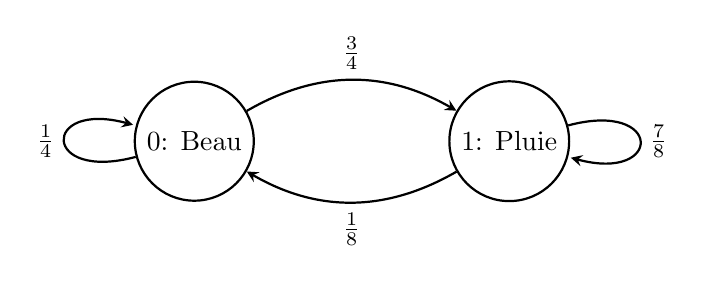
\begin{tikzpicture}[->, >=stealth, node distance=4cm, thick]
  \node[circle, draw] (B) {\( 0 \): Beau};
  \node[circle, draw, right of=B] (P) {\( 1 \): Pluie};

  \path (B) edge[loop left] node[left] {\( \frac{1}{4} \)} (B);
  \path (B) edge[bend left] node[above] {\( \frac{3}{4} \)} (P);
  \path (P) edge[loop right] node[right] {\( \frac{7}{8} \)} (P);
  \path (P) edge[bend left] node[below] {\( \frac{1}{8} \)} (B);
\end{tikzpicture}
\end{center}

La matrice de transition est :
\[
Q =
\begin{pmatrix}
\frac{1}{4} & \frac{3}{4} \\
\frac{1}{8} & \frac{7}{8}
\end{pmatrix}
\]

\subsection*{Objectif}

On note \( p(n) = \mathbb{P}(X_n = 0 \mid X_0 = 0) \), la probabilité qu’il fasse beau au jour \( n \) sachant qu’il faisait beau au jour 0.

On veut calculer :
\[
p(n) = (Q^n)_{0,0}
\]


\subsection*{Diagonalisation de la matrice}

On veut diagonaliser la matrice :
\[
Q = \begin{pmatrix}
\frac{1}{4} & \frac{3}{4} \\
\frac{1}{8} & \frac{7}{8}
\end{pmatrix}
\]

\vspace{0.5em}
\textbf{valeurs propres.}

Puisque \( Q \) est une matrice stochastique (la somme de chaque ligne vaut 1), on sait que \( \lambda_1 = 1 \) est une valeur propre.

La trace de \( Q \) est :
\[
\mathrm{Tr}(Q) = \frac{1}{4} + \frac{7}{8} = \frac{9}{8}
\]

Comme la trace d'une matrice est égale à la somme de ses valeurs propres, on a :
\[
\lambda_1 + \lambda_2 = \frac{9}{8} \quad \Rightarrow \quad \lambda_2 = \frac{9}{8} - 1 = \frac{1}{8}
\]

On a donc :
\[
\lambda_1 = 1, \quad \lambda_2 = \frac{1}{8}
\]

\vspace{0.5em}
\textbf{vecteurs propres.}

On résout \( (Q - \lambda I) v = 0 \) pour chaque valeur propre. On trouve que les vecteurs propres associés sont :
\[
v_1 = \begin{pmatrix} 1 \\ 1 \end{pmatrix}, \quad v_2 = \begin{pmatrix} -6 \\ 1 \end{pmatrix}
\]

D'où la matrice de passage :
\[
P = \begin{pmatrix} 1 & -6 \\ 1 & 1 \end{pmatrix}
\quad \text{et} \quad
P^{-1} = \begin{pmatrix} \frac{1}{7} & \frac{6}{7} \\ -\frac{1}{7} & \frac{1}{7} \end{pmatrix}
\]


La matrice diagonale associée est :
\[
D = \begin{pmatrix} 1 & 0 \\ 0 & \frac{1}{8} \end{pmatrix}
\]

Alors :
\[
Q^n = P D^n P^{-1}
\]

En multipliant :
\[
Q^n =
\begin{pmatrix}
\frac{1}{7} + \frac{6}{7}\left( \frac{1}{8} \right)^n & \frac{6}{7} - \frac{6}{7} \left( \frac{1}{8} \right)^n \\
\frac{1}{7} - \frac{1}{7} \left( \frac{1}{8} \right)^n & \frac{6}{7} + \frac{1}{7} \left( \frac{1}{8} \right)^n
\end{pmatrix}
\]

\subsection*{Résultat final}

Ainsi :
\[
\mathbb{P}(X_n = 0 \mid X_0 = 0) = p(n) = \frac{1}{7} + \frac{6}{7} \left( \frac{1}{8} \right)^n
\]

Cela signifie que la probabilité qu’il fasse beau au jour \( n \), en partant d’un jour ensoleillé, \textbf{tend vers \( \frac{1}{7} \)} lorsque \( n \to \infty \).

\section{Expecting HTH}

\subsection*{Exercice :}

\begin{exerciseBox}[Expecting HTH]
En moyenne, combien de lancers d'une pièce équilibrée (pile ou face) faut-il pour observer la séquence \textbf{HTH} (Pile–Face–Pile) pour la première fois ?
\end{exerciseBox}

\subsection*{Solution :}

\subsection*{Chaîne de Markov}

On modélise l’apparition de \texttt{HTH} à l’aide de la chaîne suivante :

\begin{itemize}
  \item $S_0$ : rien encore vu
  \item $S_1$ : on a vu \texttt{H}
  \item $S_2$ : on a vu \texttt{HT}
  \item $S_3$ : on a vu \texttt{HTH} — état absorbant
\end{itemize}

\begin{center}
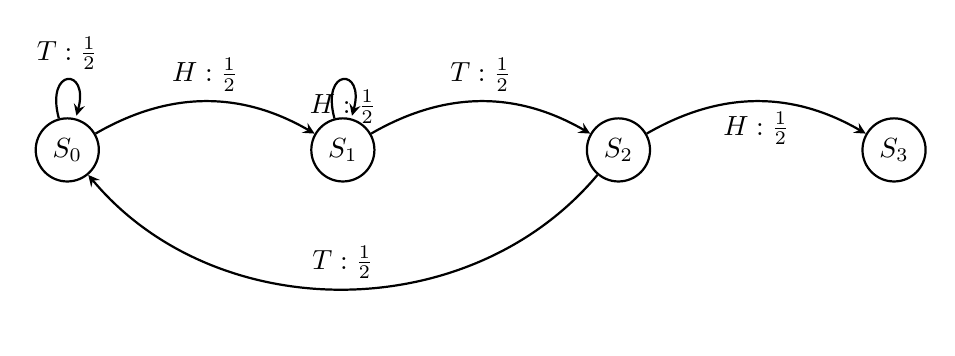
\begin{tikzpicture}[->, >=stealth, node distance=3.5cm, thick]
  \node[circle, draw] (S0) {\( S_0 \)};
  \node[circle, draw, right of=S0] (S1) {\( S_1 \)};
  \node[circle, draw, right of=S1] (S2) {\( S_2 \)};
  \node[circle, draw, right of=S2] (S3) {\( S_3 \)};

  \path (S0) edge[loop above] node {\( T:\frac{1}{2} \)} (S0);
  \path (S0) edge[bend left] node[above] {\( H:\frac{1}{2} \)} (S1);

  \path (S1) edge[bend left] node[above] {\( T:\frac{1}{2} \)} (S2);
  \path (S1) edge[loop above] node[below] {\( H:\frac{1}{2} \)} (S1);

  \path (S2) edge[bend left] node[below] {\( H:\frac{1}{2} \)} (S3);
  \path (S2) edge[bend left=50] node[above] {\( T:\frac{1}{2} \)} (S0);
\end{tikzpicture}
\end{center}

\subsection*{Système d’équations}

On cherche le temps moyen \( \mu_i \) pour atteindre \( S_3 \) à partir de \( S_i \). On a \( \mu_3 = 0 \). Le système est :

\[
\begin{cases}
\mu_0 = 1 + \frac{1}{2} \mu_0 + \frac{1}{2} \mu_1 \\
\mu_1 = 1 + \frac{1}{2} \mu_1 + \frac{1}{2} \mu_2 \\
\mu_2 = 1 + \frac{1}{2} \cdot 0 + \frac{1}{2} \mu_0 = 1 + \frac{1}{2} \mu_0
\end{cases}
\]

\subsection*{Résolution}

Équation 3 : \( \mu_2 = 1 + \frac{1}{2} \mu_0 \)

Substituer dans 2 :
\[
\mu_1 = 1 + \frac{1}{2} \mu_1 + \frac{1}{2}(1 + \frac{1}{2} \mu_0)
= 1 + \frac{1}{2} \mu_1 + \frac{1}{2} + \frac{1}{4} \mu_0
= \frac{3}{2} + \frac{1}{2} \mu_1 + \frac{1}{4} \mu_0
\]
\[
\Rightarrow \mu_1 - \frac{1}{2} \mu_1 = \frac{3}{2} + \frac{1}{4} \mu_0
\Rightarrow \frac{1}{2} \mu_1 = \frac{3}{2} + \frac{1}{4} \mu_0
\Rightarrow \mu_1 = 3 + \frac{1}{2} \mu_0
\]

Substituer dans 1 :
\[
\mu_0 = 1 + \frac{1}{2} \mu_0 + \frac{1}{2}(3 + \frac{1}{2} \mu_0)
= 1 + \frac{1}{2} \mu_0 + \frac{3}{2} + \frac{1}{4} \mu_0
= \frac{5}{2} + \frac{3}{4} \mu_0
\]
\[
\Rightarrow \mu_0 - \frac{3}{4} \mu_0 = \frac{5}{2}
\Rightarrow \frac{1}{4} \mu_0 = \frac{5}{2}
\Rightarrow \mu_0 = 10
\]

\subsection*{Conclusion}

Le temps moyen d’apparition de la séquence \texttt{HTH} est :

\[
\boxed{10}
\]

